\chapter{Anwendungsbeispiel}

Das folgende Beispiel ist mit der statistischen Software \texttt{R} (\citealp{R}) und dem Zusatzpaket \texttt{svmpath} (\citealp{svmpath}) erstellt worden. Der dazugeh�rige R-Code befindet sich in der mitgelieferten Datei \texttt{Anwendungsbeispiel.R}. Eine weitere Umsetzung f�r Support Vector Machines in \texttt{R} ist unter anderem in der Funktion 
%\texttt{ksvm()} aus dem Paket \texttt{kernlab} \citep{kernlab} oder in der Funktion 
\texttt{svm()} aus dem Paket \texttt{e1071} (\citealp{e1071}) zu finden.

Zun�chst werden $200$ Beobachtungen simuliert, die dann durch zuf�lliges Ziehen im Verh�ltnis von $4:1$ in Trainingsdaten und Testdaten aufgeteilt werden. 
Die $N=160$ Trainingsdaten in Abbildung \ref{train} sollen das Zwei-Spiralen-Problem in einem zweidimensionalen Variablenraum nachstellen. Dabei handelt es sich um ein bekanntes bin�res Klassifikationsproblem, bei dem die zwei Klassen spiralf�rmig miteinander verzahnt sind.

\begin{figure}[h]
\centering
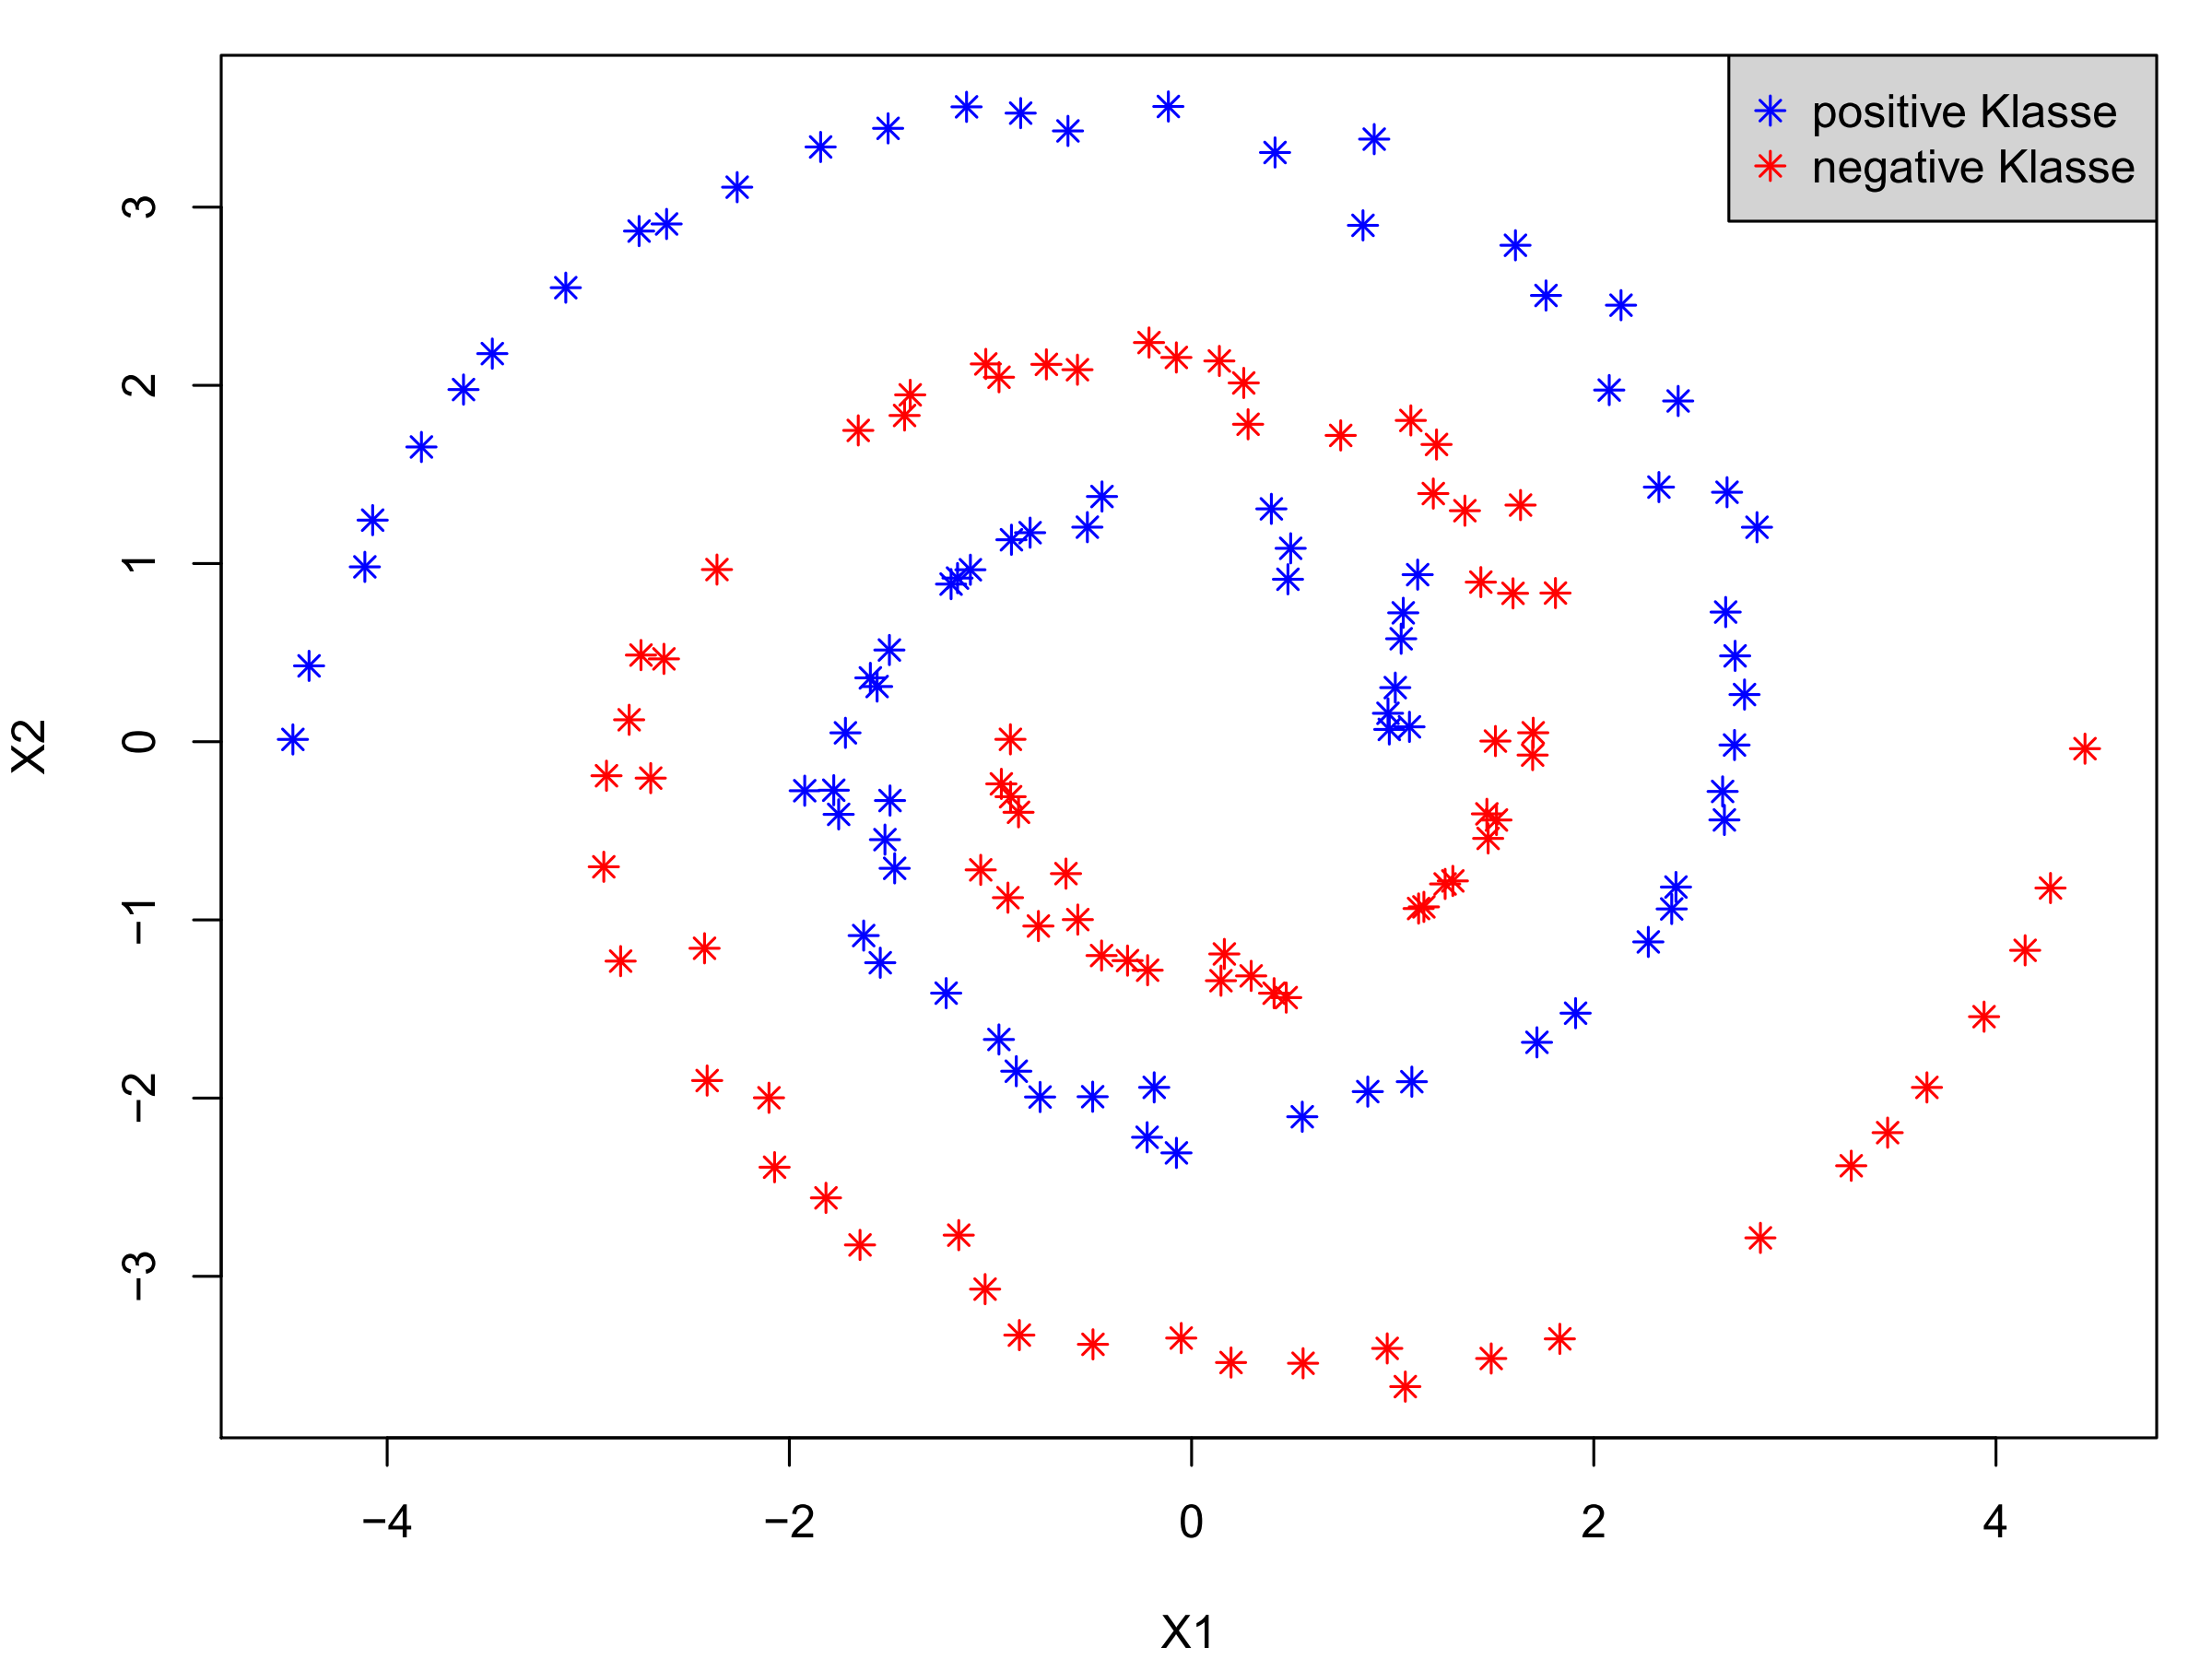
\includegraphics[width=\textwidth]{traintest_01.png}
\caption{Spiralf�rmige Trainingsdaten}
\label{train}
\end{figure}

Gesucht ist eine Hyperebene, welche die Trainingsdaten f�r m�glichst viele Beobachtungen voneinander trennt. Die Testdaten sollen anschlie�end, durch die auf Basis der Trainingsdaten gesch�tzten Hyperebene, m�glichst fehlerfrei in die beiden Klassen zugeordnet werden.

In Abbildung \ref{polyKern} wurde die Hyperebene durch Verwendung einer polynomialen Kernfunktion zweiten Grades der Form $K(\mathbf{x}_i,\mathbf{x}_j) = (\mathbf{x}_i^\top \mathbf{x}_j + 1)^2$ ermittelt. Im Vergleich dazu wurde in Abbildung \ref{rbfKern} als Kernfunktion eine gau�sche radiale Basisfunktion (RBF) der Form $K(\mathbf{x}_i,\mathbf{x}_j) = \exp(-||\mathbf{x}_i-\mathbf{x}_j||)$ verwendet.

\begin{figure}[h]
\begin{minipage}[b]{0.5\linewidth}
\centering
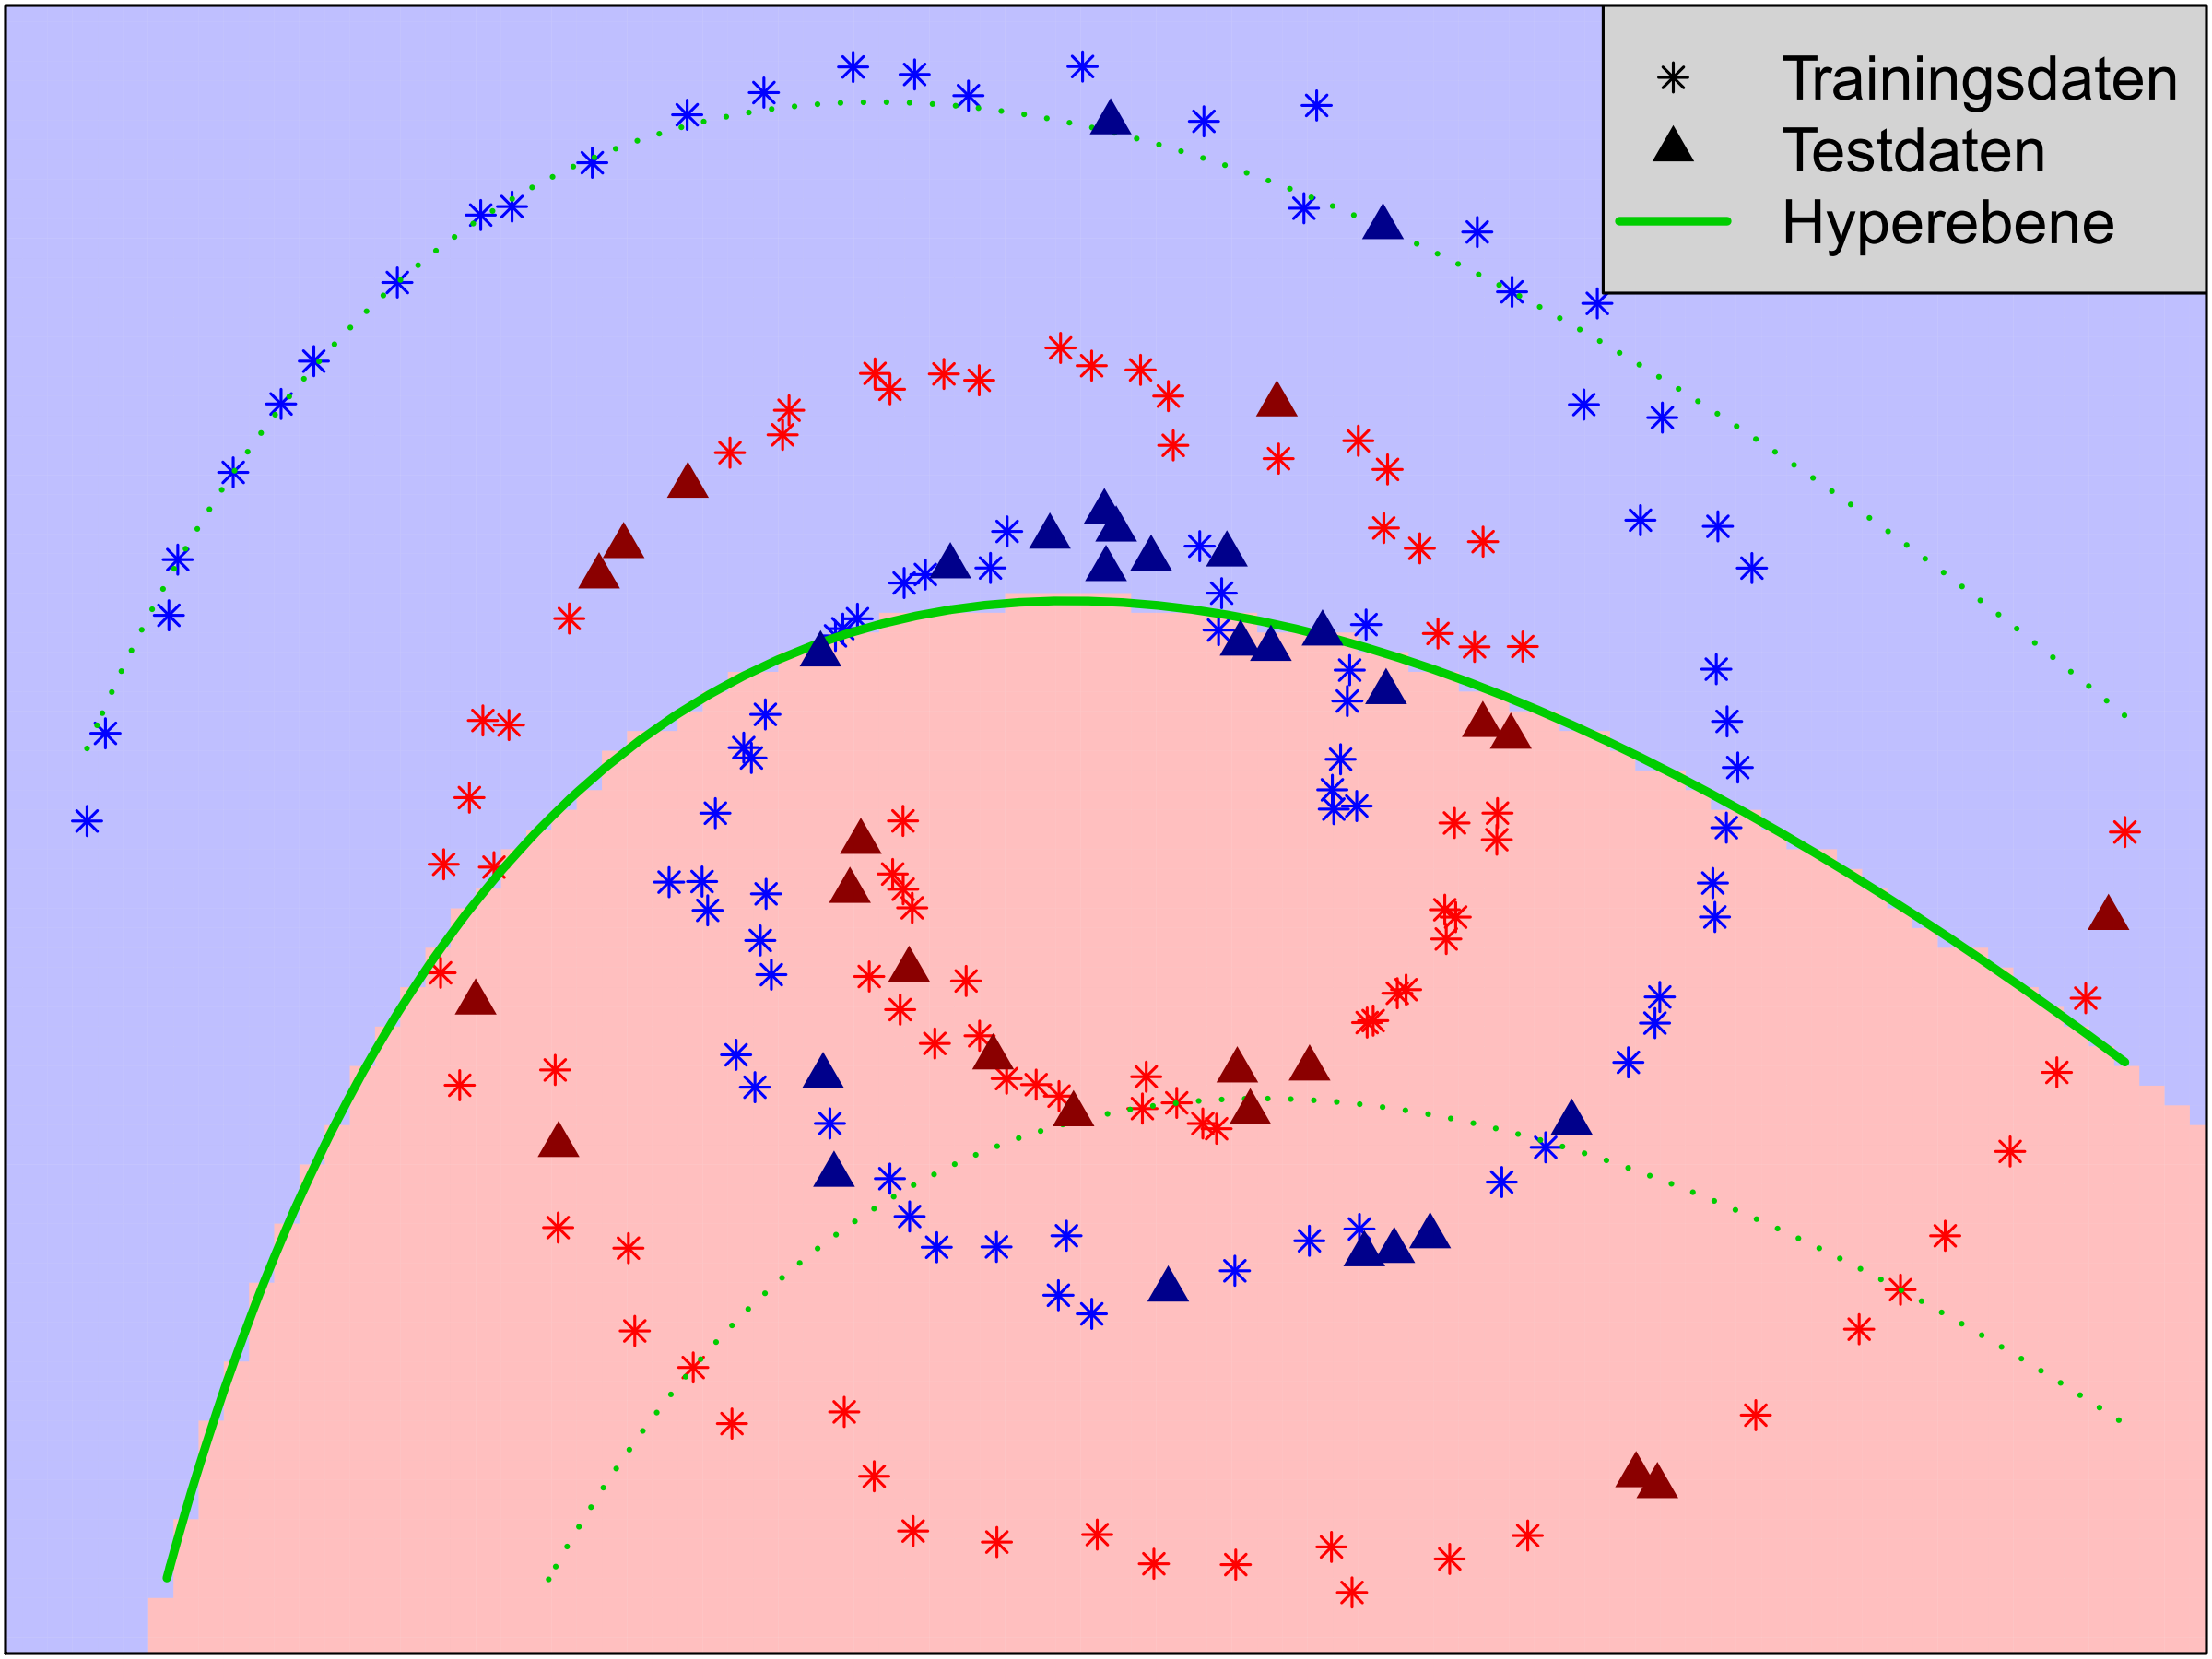
\includegraphics[width=\textwidth]{traintest_03.png}
\caption{polynomiale Kernfunktion}
\label{polyKern}
\end{minipage}
\hspace{0.1cm}
\begin{minipage}[b]{0.5\linewidth}
\centering
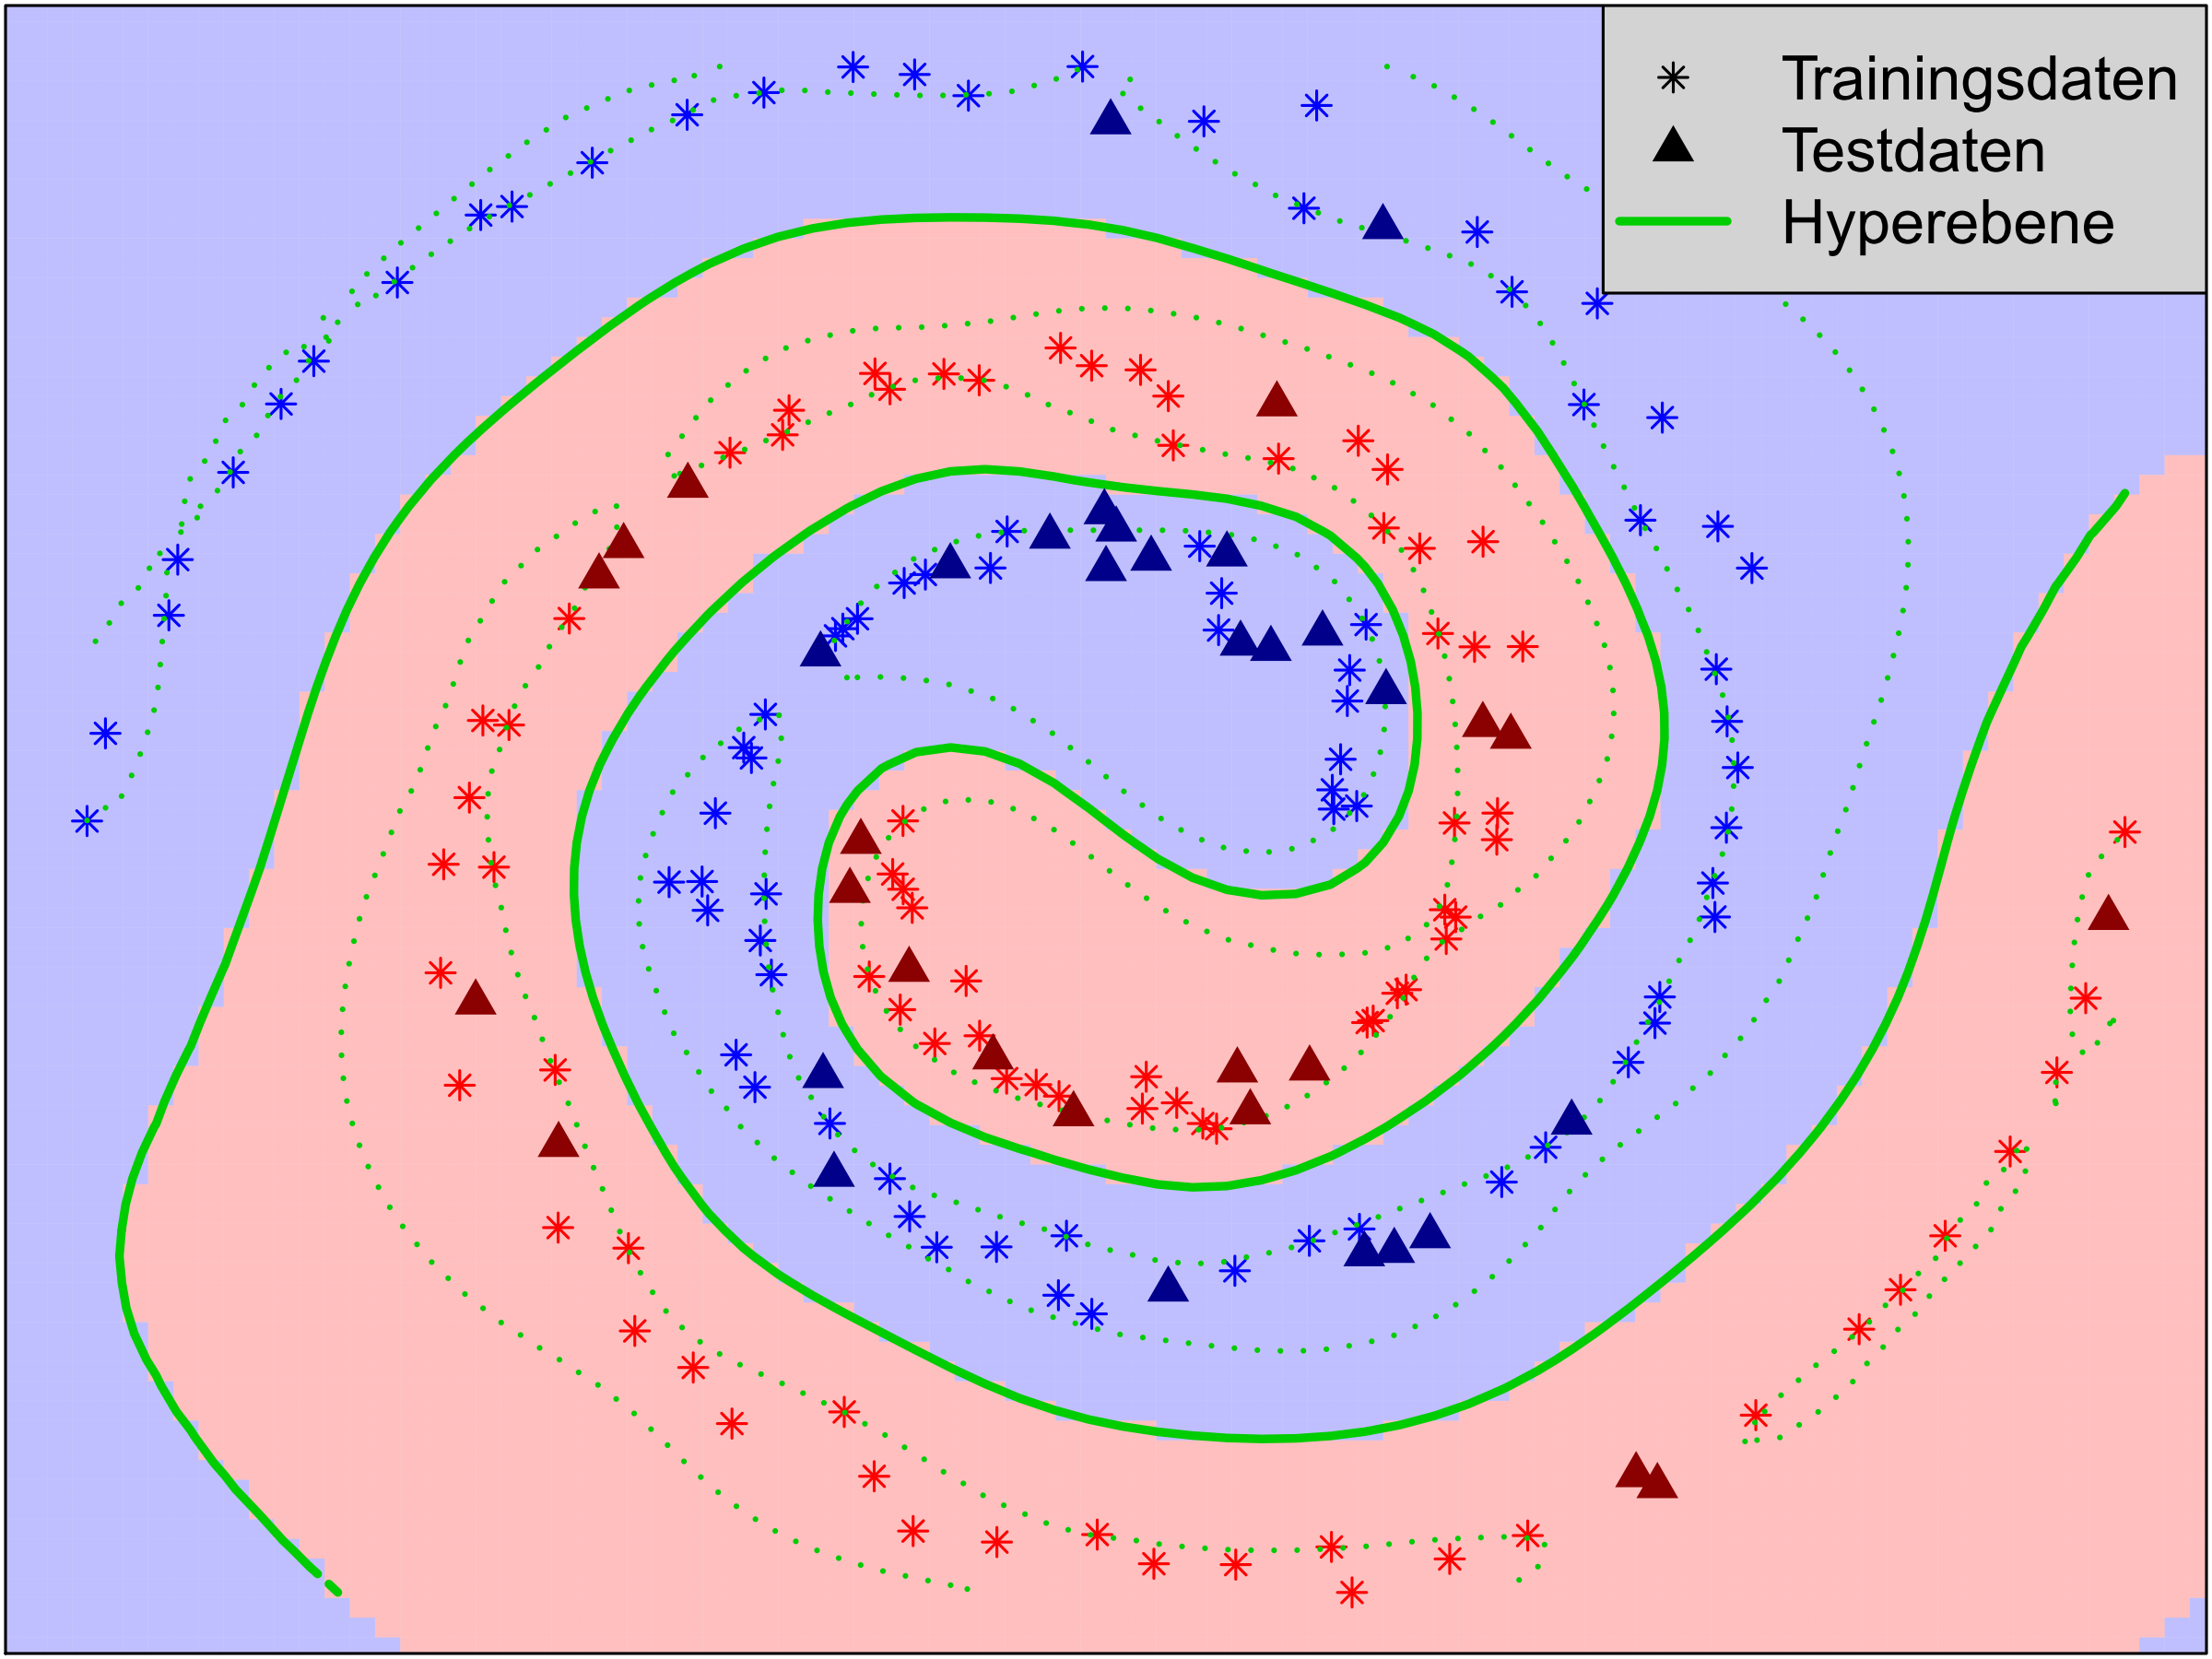
\includegraphics[width=\textwidth]{traintest_02.png}
\caption{gau�sche RBF}
\label{rbfKern}
\end{minipage}
\end{figure}

%\begin{figure}[h]
%\centering
%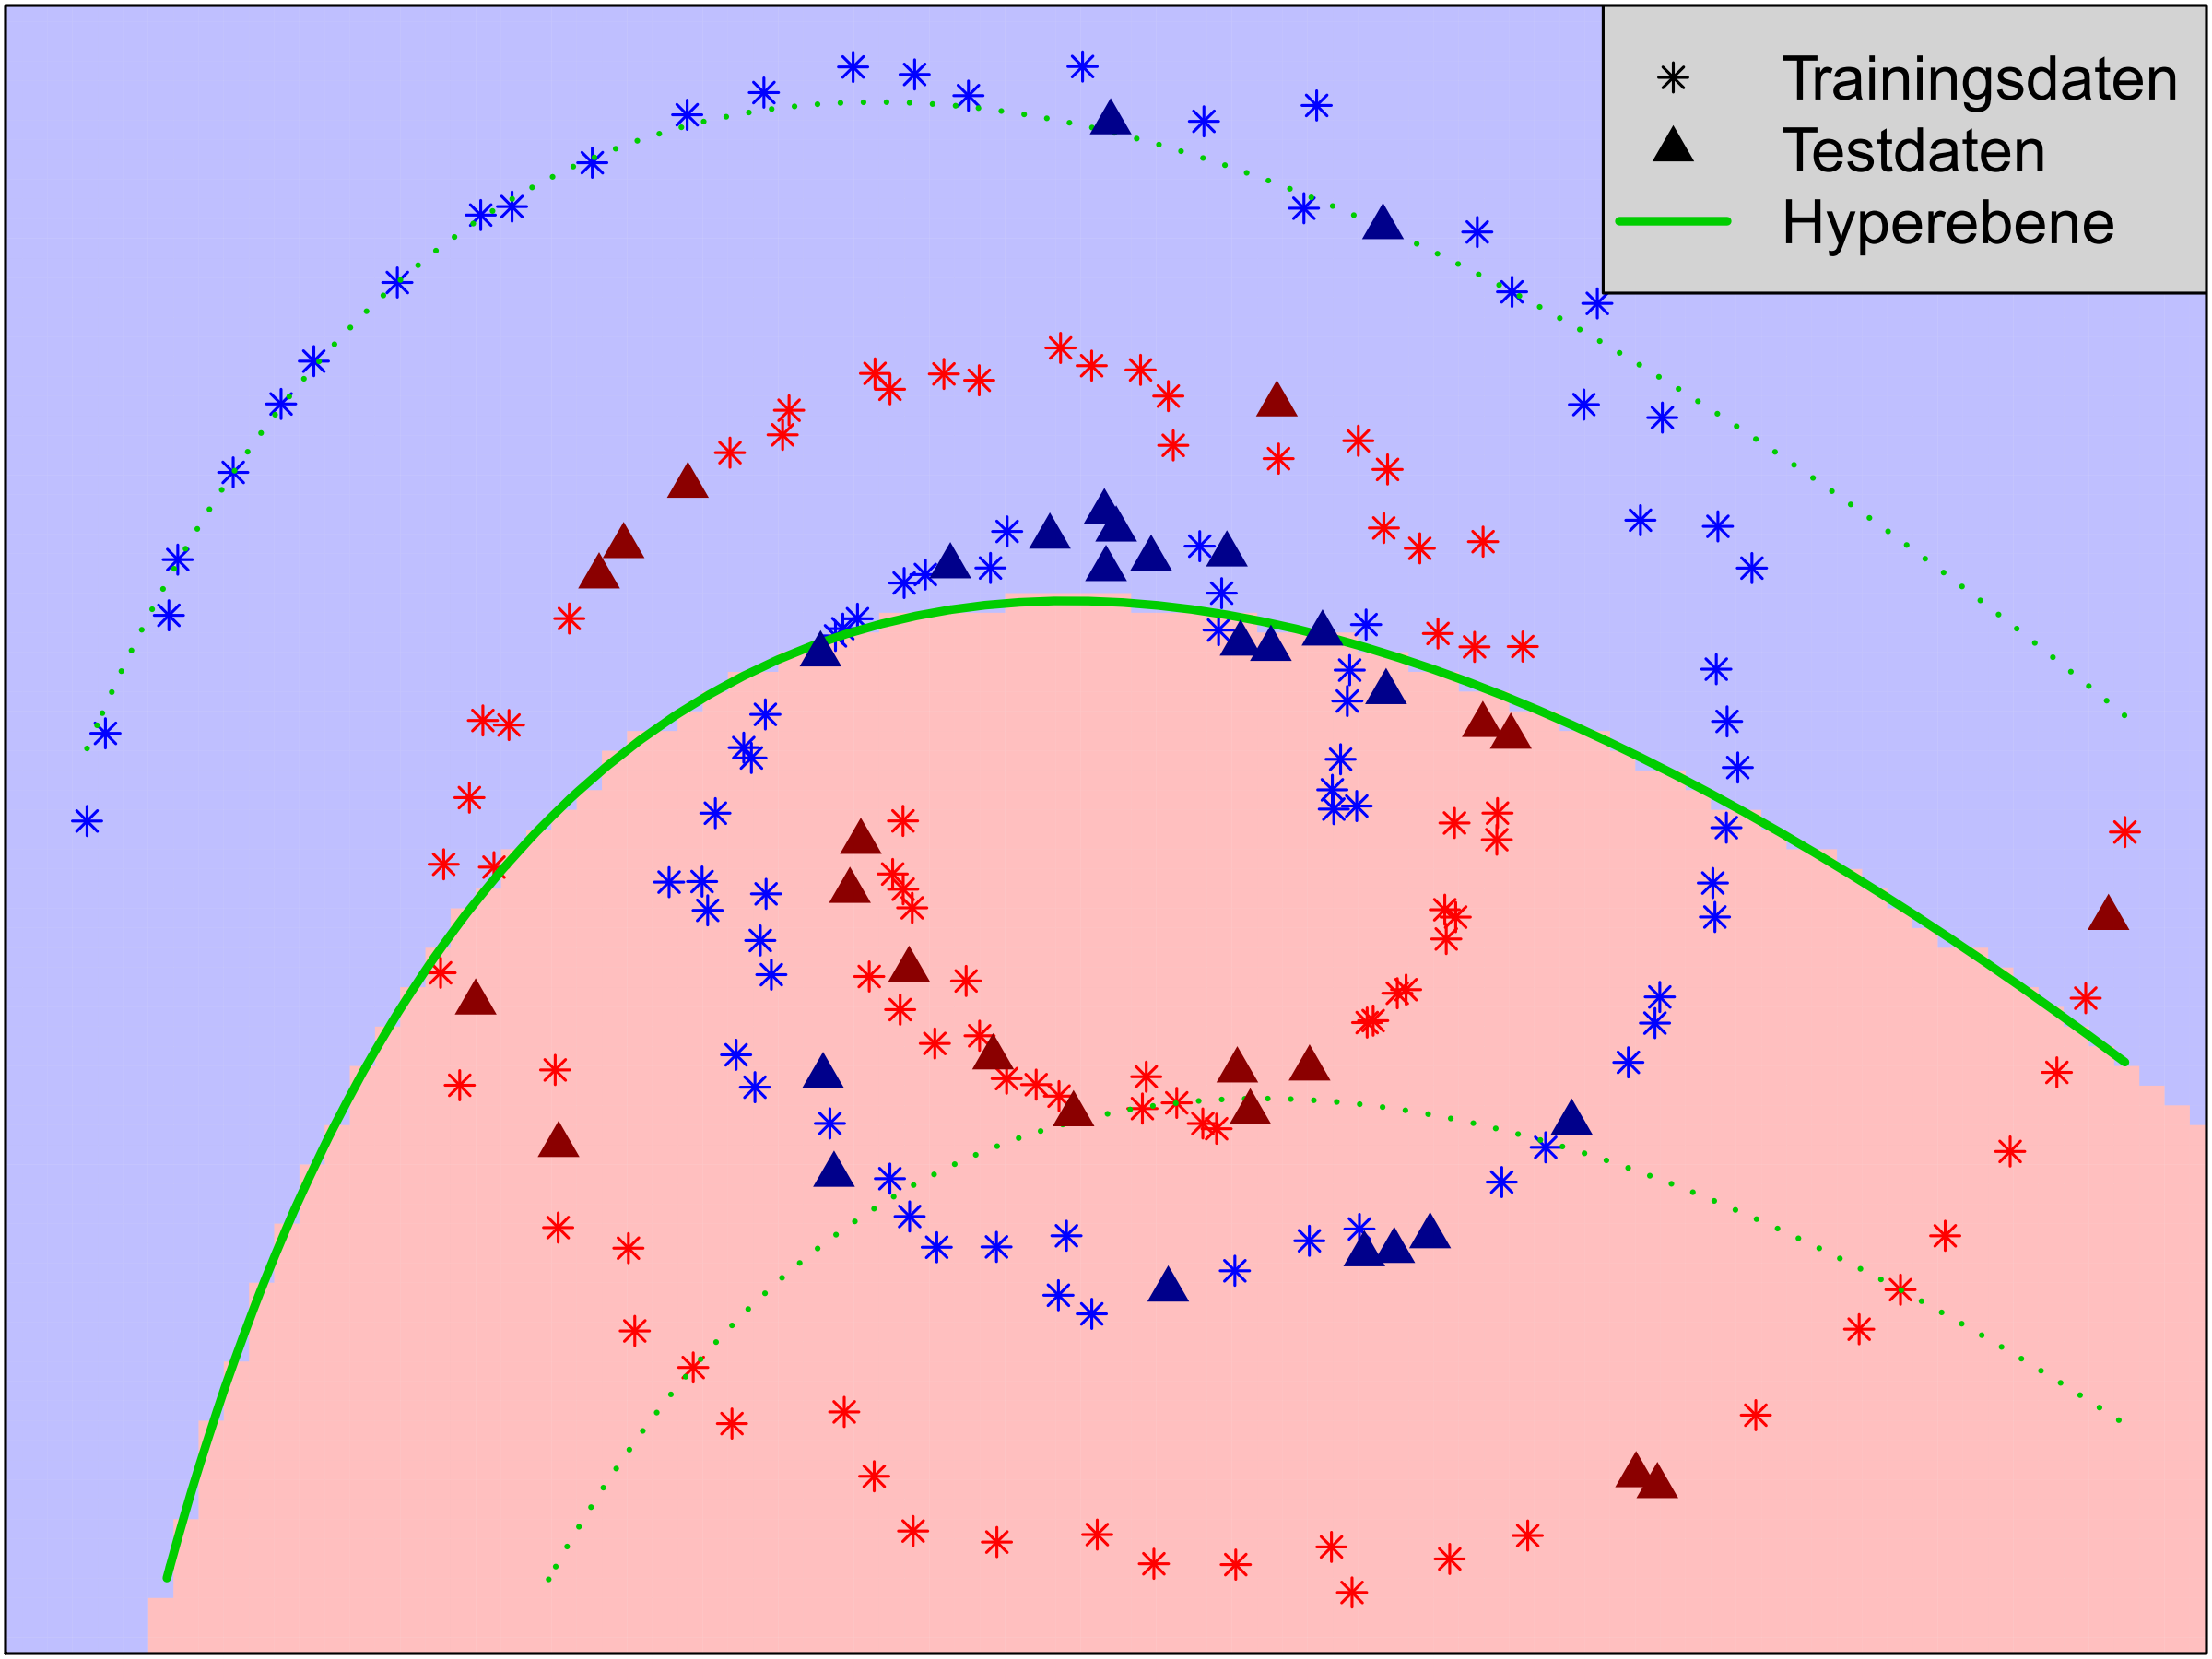
\includegraphics[width=0.6\textwidth]{traintest_03.png}
%\caption{polynomiale Kernfunktion}
%\label{polyKern}
%\end{figure}
%\begin{figure}[h]
%\centering
%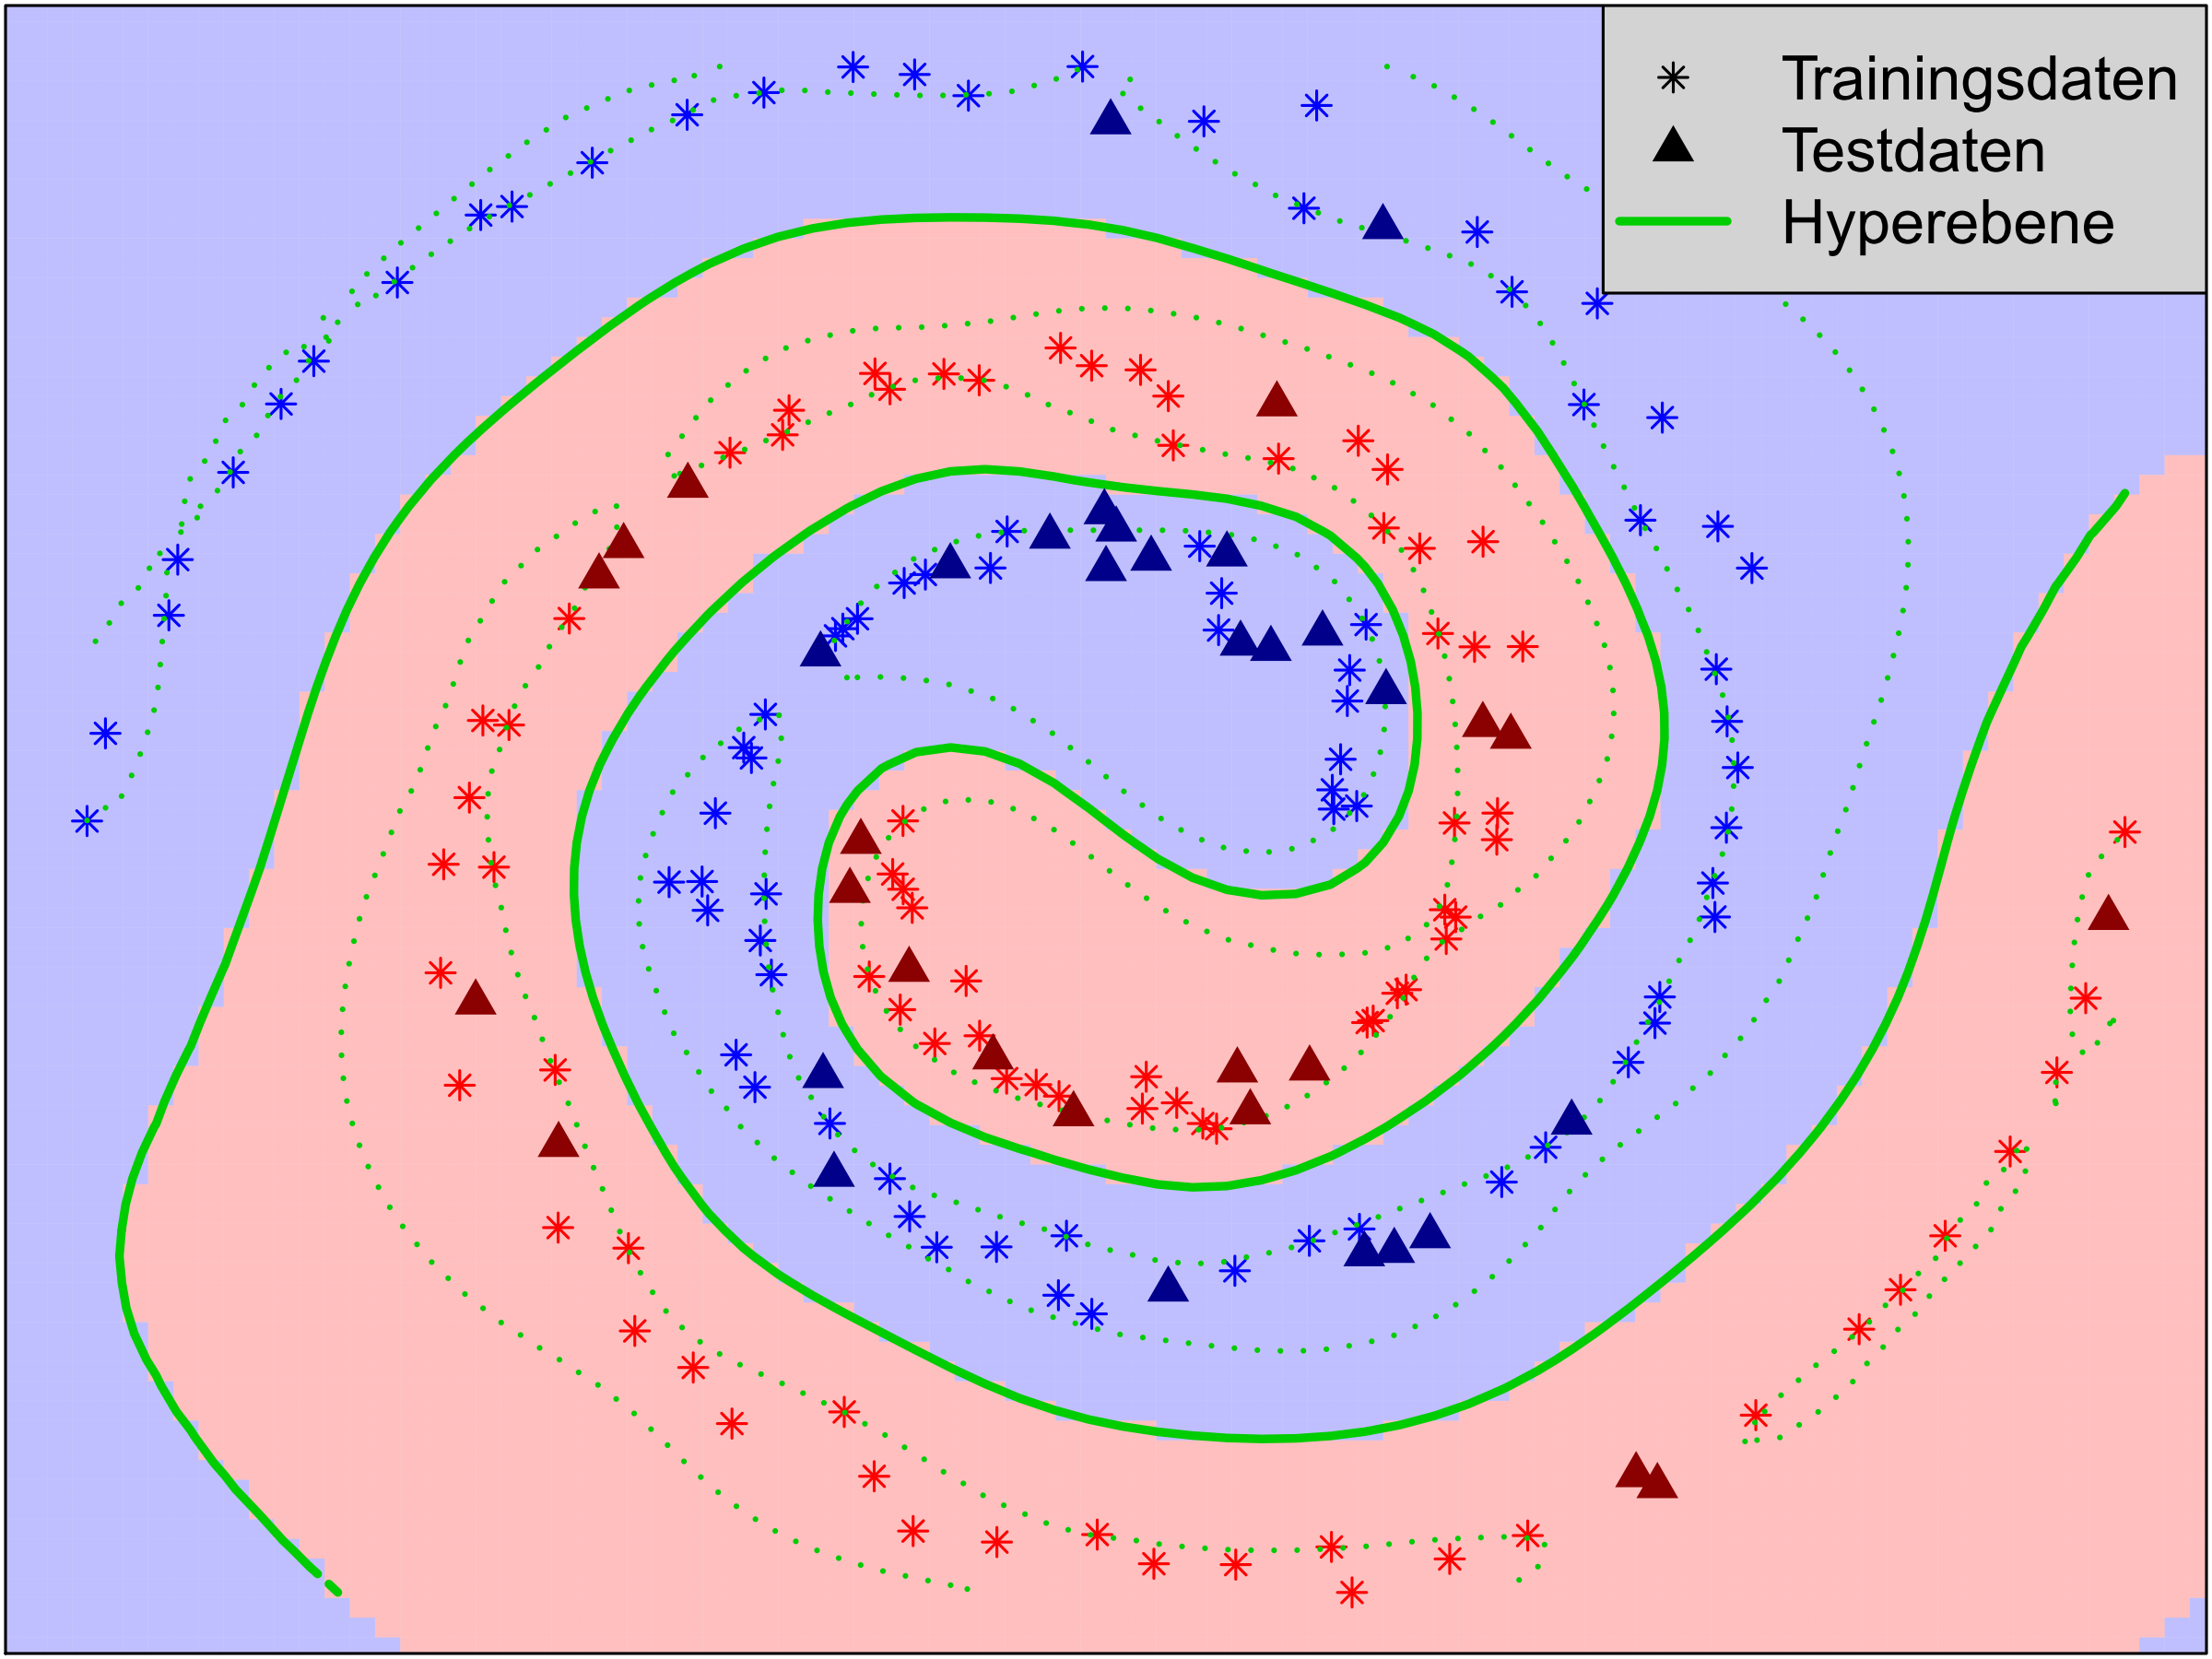
\includegraphics[width=0.6\textwidth]{traintest_02.png}
%\caption{gau�sche RBF}
%\label{rbfKern}
%\end{figure}

%Hier sieht man dass die polynomiale Kernfunktion wieder einer Ellipse entspricht Wie in Kapitel \ref{sec:kerneltrick} erl�ute
Die polynomiale Kernfunktion kann die spiralf�rmig verzahnten Trainingsdaten hier nicht vollst�ndig voneinander trennen, da die resultierenden Hyperebenen die Form eines Kegelschnitts haben (vgl. Kapitel \ref{sec:kerneltrick}). Die gau�sche radiale Basisfunktion hingegen �berf�hrt den Variablenraum in einen hochdimensionalen Variablenraum, bei dem eine Hyperebene gefunden werden kann, welches die Trainingsdaten vollst�ndig voneinander trennt. 
Tabelle \ref{tab:missclass} zeigt dabei die Anzahl bzw. den Anteil der fehlklassifizierten Trainingsdaten und Testdaten.

\begin{table}[ht]
\begin{center}
\begin{tabular}{|c||c|c||c|c|}
\hline 
 & \multicolumn{2}{c||}{Trainingsdaten} & \multicolumn{2}{c|}{Testdaten}\\ %\hline
 & Anzahl & Anteil & Anzahl & Anteil \\ 
  \hline
Abbildung \ref{polyKern} & 67 &  41.875 \% &    16 & 40 \% \\ 
   \hline
Abbildung \ref{rbfKern}  & 0 & 0 \% & 0 & 0 \% \\ 
   \hline
\end{tabular}
\end{center}
\caption{Fehlklassifizierungen in Trainingsdaten und Testdaten}
\label{tab:missclass}
\end{table}

%bla \ref{tab:label}
%\begin{table}[t]
%\centering
%\begin{tabular}{c|c}
%4	& 5\\ %table content
%\end{tabular}
%\caption{ba}
%\label{tab:label}
%\end{table}